\documentclass{standalone}
\usepackage{tikz}
\usepackage{amssymb}
\usepackage{amsmath}
\usepackage{amstext}
\usepackage{xcolor}
\usetikzlibrary{positioning,shapes.geometric}
\usetikzlibrary{arrows}
\begin{document}

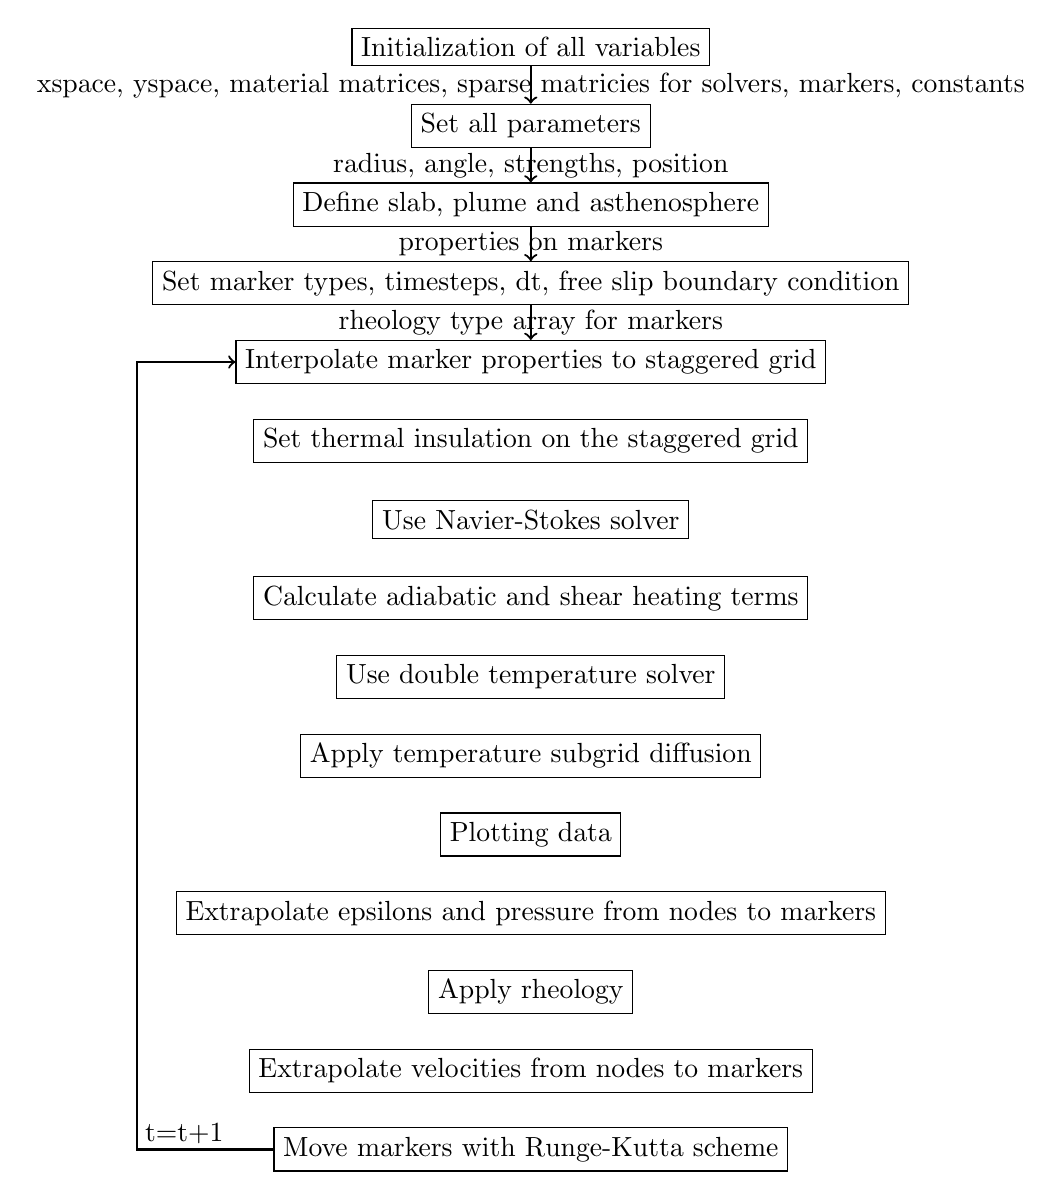
\begin{tikzpicture}[
	  scale=1.0,
	  %style for arrows
	  arrw/.style={thick, ->, >=to},
      % fisrt style for boxes      
      op/.style={rectangle, fill=black!15, draw=black},
      % second style for boxes
      dt/.style={rectangle, fill=white, draw=black}]
            
      %nodes
      \node[dt](initdom){Initialization of all variables};
      \node[dt,below of=initdom](setparams){Set all parameters};
      \node[dt,below of=setparams](geometry){Define slab, plume and asthenosphere};
      \node[dt,below of=geometry](markers){Set marker types, timesteps, dt, free slip boundary condition};
      
      \node[dt,below of=markers](startinterpol){Interpolate marker properties to staggered grid};
      \node[dt,below of=startinterpol](deftemp){Set thermal insulation on the staggered grid};
      \node[dt,below of=deftemp](navierstokes){Use Navier-Stokes solver};
      \node[dt,below of=navierstokes](heatingterms){Calculate adiabatic and shear heating terms};
      \node[dt,below of=heatingterms](tempsolver){Use double temperature solver};
      \node[dt,below of=tempsolver](tempdiff){Apply temperature subgrid diffusion};
      \node[dt,below of=tempdiff](fig){Plotting data};
      \node[dt,below of=fig](extrapolation){Extrapolate epsilons and pressure from nodes to markers};
      \node[dt,below of=extrapolation](rheology){Apply rheology};
      \node[dt,below of=rheology](extrapolvelocity){Extrapolate velocities from nodes to markers};
      \node[dt,below of=extrapolvelocity](rungekutta){Move markers with Runge-Kutta scheme};
      %edges
	  \draw[arrw](rungekutta) -- ++(-5,0)-| node[xshift=0.6cm,yshift=0.2cm]{t=t+1} ++(0,6)|- (startinterpol);
	  \draw[arrw](initdom)--node{xspace, yspace, material matrices, sparse matricies for solvers, markers, constants}(setparams);
	  \draw[arrw](setparams) -- node{radius, angle, strengths, position} (geometry);
	  \draw[arrw](geometry) --node{properties on markers} (markers);
	  \draw[arrw](markers) --node{rheology type array for markers} (startinterpol);
\end{tikzpicture}
  
\end{document}